\documentclass{jarticle}
\usepackage[dvipdfmx]{graphicx}
\usepackage{here}

\title{{システム実験}\\基礎実験1}
\author{6119019056 山口力也}
\date{2019/04/19日提出}

\begin{document}
\maketitle

\section{概要}
本実験では,これからシステム実験を行う上で知っておくべき部品の基礎知識,マイコンの動作原理,Arduino UNOの使用方法を習得することを目的とした.基礎実験の達成目標を次に示す.

\begin{itemize}

\item 電子回路部品の基礎知識や基本特性を習得する.
\item 電子回路をブレッドボード上に作成できる.
\item マイコンの動作原理について理解する.
\item Arduinoと周辺回路を適切に接続できる.
\item Arduinoの基本機能(IO,AD,PWM,割り込み,タイマ,シリアル通信等)を理解して,使いこなせる.

\end{itemize}

\section{実験内容}
\subsection{抵抗のカラーコードと抵抗値}
\label{subsec:colorcode}
演習として抵抗のカラーコードを読み抵抗値を調べた.また,課題として6種類の異なる抵抗値をカラーコードに変換を行った.
\subsection{LEDの点灯}
\label{subsec:led}
演習としてまずLEDの極性(アノード・カソード)を確認した.その後Arudinoを用いてブレッドボード上にLED点灯回路を作成し,課題としてLEDの色を黄色,緑に変更し動作を確認した.また抵抗を330$\Omega$,510$\Omega$,1k$\Omega$,10k$\Omega$,1M$\Omega$に変更してそれぞれでのLEDに流れる電流を計算し,発光状態を確認した.

\subsubsection{合成抵抗によるLEDの点灯1}
\label{subsubsec:gouseiled1}
課題として図\ref{fig:gouseiteikou}を参考に330$\Omega$,510$\Omega$,1k$\Omega$の抵抗から2つの抵抗を選び,組み合わせて抵抗値が840$\Omega$になるように合成抵抗をブレッドボード上で実装し,電流制限抵抗として用い赤色LEDを点灯させた.また,その時LEDに流れる電流を計算し,LEDの発光状態を確認した.

\begin{figure}[H]
\begin{center}
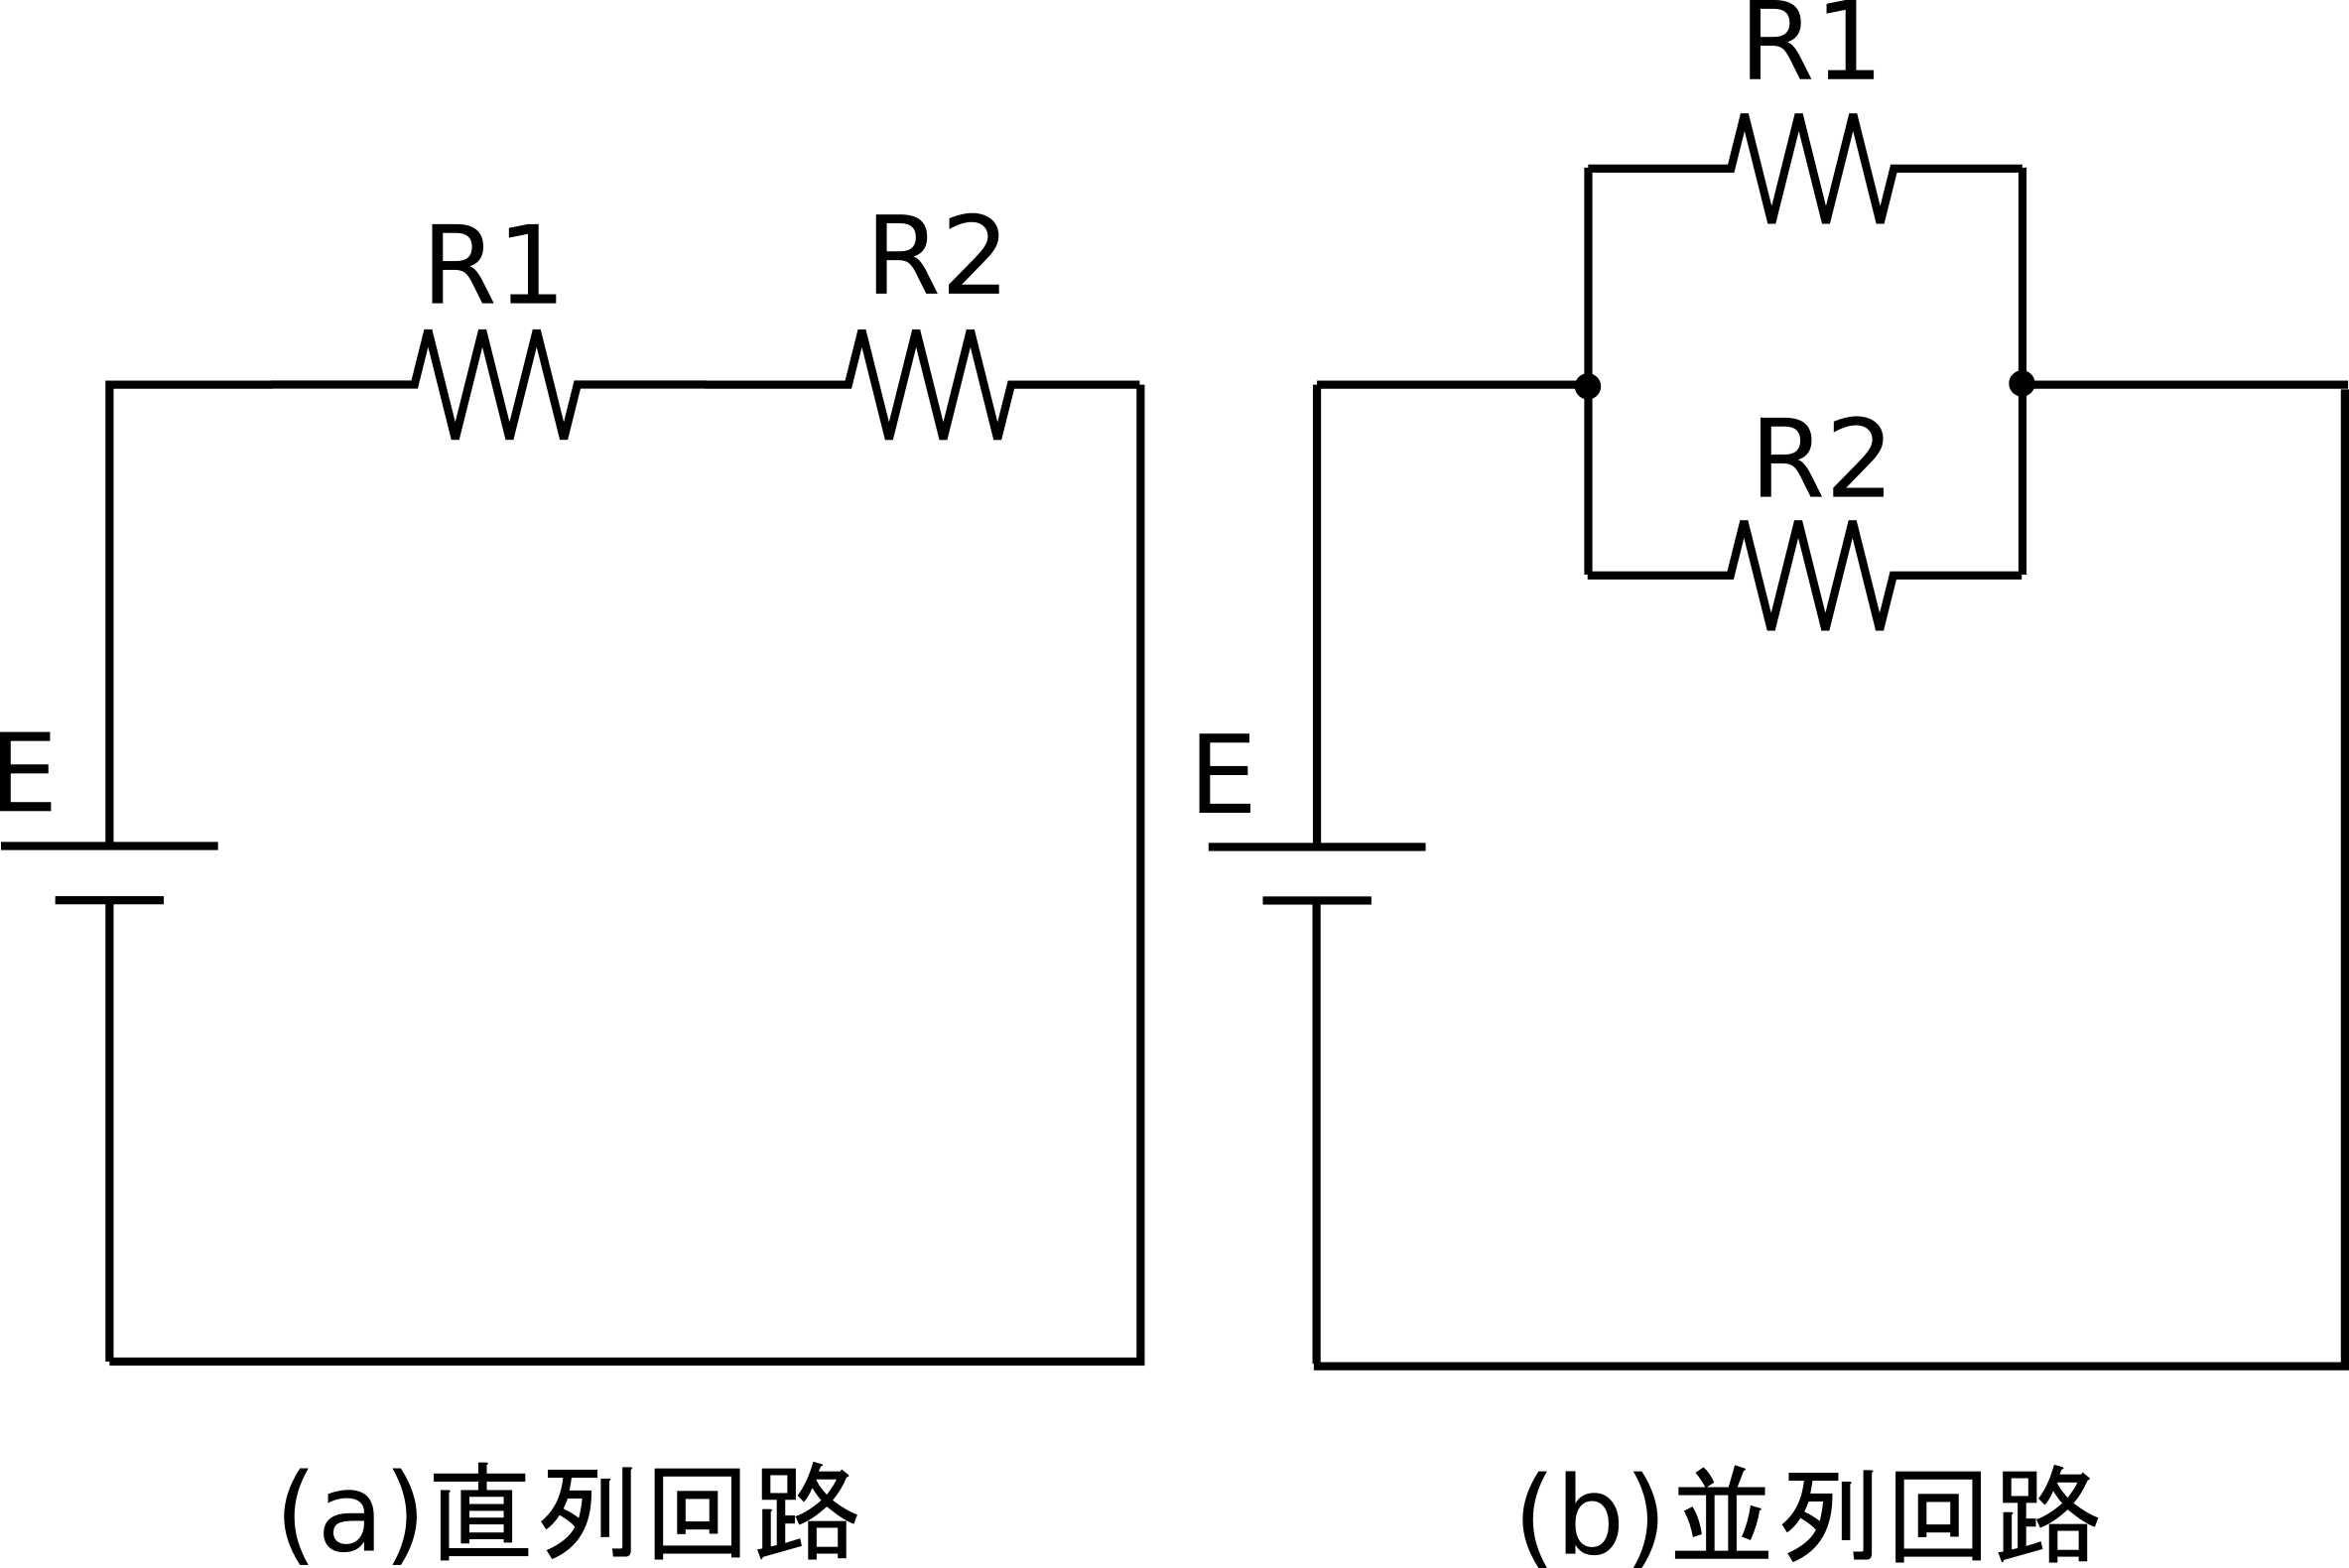
\includegraphics[width=7.0cm]{images/kairo.png}
\caption{合成抵抗の回路(例)}
\label{fig:gouseiteikou}
\end{center}
\end{figure}

\subsubsection{合成抵抗によるLEDの点灯2}
\label{subsubsec:gouseiled2}
課題として図\ref{fig:gouseiteikou}を参考に330$\Omega$,510$\Omega$,1k$\Omega$の抵抗から2つの抵抗を選び,組み合わせて抵抗値が約200$\Omega$になるように合成抵抗をブレッドボード上で実装し,電流制限抵抗として用い赤色LEDを点灯させた.また,その時LEDに流れる電流を計算し,LEDの発光状態を確認した.

\subsection{タクトスイッチによる制御}
\label{subsec:switch}
演習として,タクトスイッチを用いたLED点灯回路の回路図を作成し,課題としてタクトスイッチを用いたLED点灯回路を作成した.また,タクトスイッチを2つ(SW1,SW2)用いてそれぞれ以下の表\ref{table:and},表\ref{table:or}を満たすスイッチのON,OFF動作を行う回路を作成した.

\begin{table}[H]
\centering
\caption{条件1}
\label{table:and}
\begin{center}
\begin{tabular}{c|c|c}
\hline \hline
SW1 & SW2 & LEDの状態\\ \hline
ON & ON &点灯 \\
ON& OFF & 消灯 \\
OFF& ON& 消灯\\
OFF& OFF & 消灯\\ \hline
\end{tabular}
\end{center}
\end{table}

\begin{table}[H]
\centering
\caption{条件2}
\label{table:or}
\begin{center}
\begin{tabular}{c|c|c}
\hline \hline
SW1 & SW2 & LEDの状態\\ \hline
ON & ON &点灯 \\
ON& OFF & 点灯 \\
OFF& ON& 点灯\\
OFF& OFF & 消灯\\ \hline
\end{tabular}
\end{center}
\end{table}

\subsection{[発展課題1]合成抵抗}
\label{subsec:hatten1}
6種類の抵抗(75$\Omega$330$\Omega$,510$\Omega$,1k$\Omega$,10k$\Omega$,1M$\Omega$)から3つの抵抗を選択し,670$\Omega$の合成抵抗を作成した.またその合成抵抗を電流制限抵抗として用い,赤色LEDを点灯させる回路をブレッドボード上に作成した.

\subsection{[発展課題2]RGBフルカラーLEDの点灯}
\label{subsec:hatten2}
RGBフルカラーLEDを点灯させる回路をブレッドボード上に作成した.ここで,赤,緑,青,それぞれのLEDの電流制限抵抗R=1k$\Omega$を使用した.


\section{実験結果}
\subsection{抵抗のカラーコードと抵抗値}
実験\ref{subsec:colorcode}の結果を以下表\ref{table:colorcode}に示す.

\begin{table}[H]
\centering
\caption{抵抗値とカラーコード}
\label{table:colorcode}
\begin{center}
\begin{tabular}{c|c}
\hline \hline
抵抗値[$\Omega$] & カラーコード \\ \hline
75 &紫(7)緑(5)黒(0)金(5\%)\\ 
330 &橙(3)橙(3)茶(1)金(5\%)  \\ 
510 &緑(5)茶(1)茶(1)金(5\%) \\ 
1k & 茶(1)黒(0)赤(2)金(5\%) \\ 
10k &茶(1)黒(0)橙(3)金(5\%)  \\ 
1M & 茶(1)黒(0)緑(5)金(5\%) \\ \hline
\end{tabular}
\end{center}
\end{table}

\subsection{LEDの極性}
以下にLEDの極性の確認の仕方を説明する.
LEDには極性(アノード,カソード)がある.極性の確認の仕方は

\begin{itemize}

\item リード線の長さ
\item パッケージの切り欠き
\item パッケージ内の形状

\end{itemize}

の3つがある.リード線の長さで判断する方法リード線が長いほうがアノード,リード線が短いほうがカソードとなっている.
パッケージの切り欠きで判断する方法では,パッケージの切り欠きがある方がカソードでありこのような目印はカソードインデクスと呼ばれる.最後のパッケージ内の形状で判断する方法では,パッケージ内のリード線の形状が大きいほうがカソード,小さいほうがアノードである.ただしまれに逆のものが存在するので注意が必要である.

\subsection{LEDの点灯}
実験\ref{subsec:led}で作成したLED点灯回路のブレッドボードの配線図および回路図を以下図\ref{fig:2-1-2bread},図\ref{fig:2-1-2kairo}に,5種類の抵抗に変更した時のLEDの発光状態を以下表\ref{table:led}に示す.
ここで,電流の計算は以下の式\ref{eq:denryu}を用いた.

\begin{equation}
I=\frac{V}{R}=\frac{5.0-2.0}{R}=\frac{3.0}{R}
\label{eq:denryu}
\end{equation}

\begin{table}[H]
\centering
\caption{LEDの点灯}
\label{table:led}
\begin{center}
\begin{tabular}{c|c|c}
\hline \hline
抵抗値[$\Omega$] &LEDに流れる電流[mA] &LEDの発光状態\\ \hline
330&9.09&明るい\\
510&5.88&明るい\\
1k&3.00&やや暗い\\
10k&0.3&暗い\\
1M&0.003&点灯しない\\ \hline
\end{tabular}
\end{center}
\end{table}

\begin{figure}[H]
\begin{center}
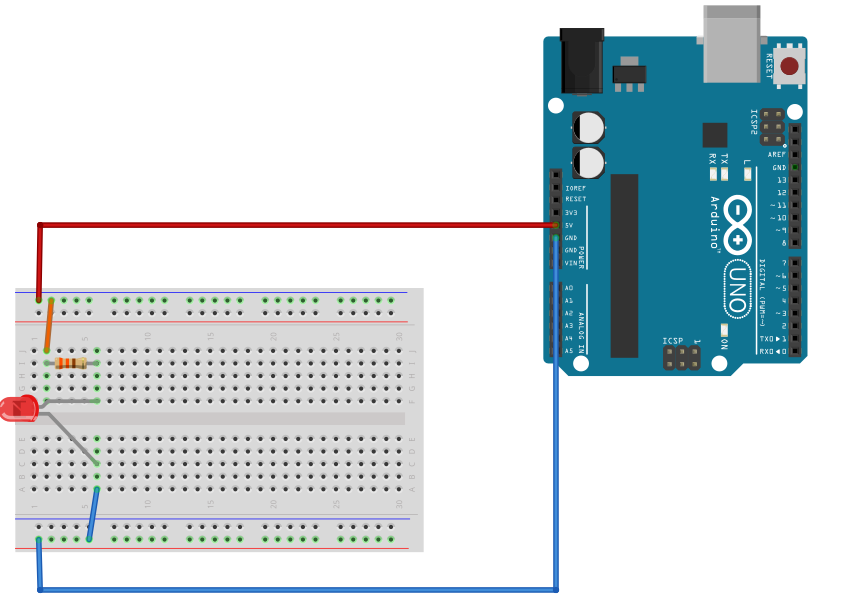
\includegraphics[width=8.0cm]{images/kadai2-1-2_ブレッドボード.png}
\caption{LED点灯回路の配線図}
\label{fig:2-1-2bread}
\end{center}
\end{figure}

\begin{figure}[H]
\begin{center}
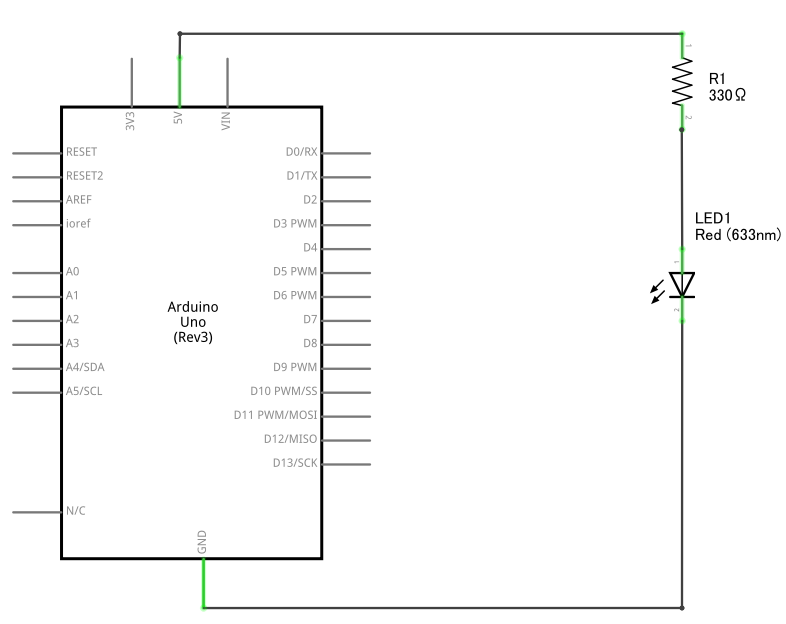
\includegraphics[width=7.0cm]{images/kadai2-1-2_回路図.png}
\caption{LED点灯回路の回路図}
\label{fig:2-1-2kairo}
\end{center}
\end{figure}

表\ref{table:led}のように光の強さが異なるのは,電流制限抵抗の値が変化することでLEDに流れる電流が変わるためだと考えられる.電流制限抵抗を大きくすると式\ref{eq:denryu}よりLEDに流れる電流が少なくなり,光の強度が小さくなる.

\subsection{合成抵抗によるLED点灯}
実験\ref{subsubsec:gouseiled1}の結果を以下表\ref{table:gouseiled1}に,実験\ref{subsubsec:gouseiled2}の結果を以下表\ref{table:gouseiled2}に示す.

\begin{table}[H]
\centering
\caption{合成抵抗によるLED点灯1}
\label{table:gouseiled1}
\begin{center}
\begin{tabular}{c|c|c|c|c|c}
\hline \hline
種類 & 抵抗R1[$\Omega$] & 抵抗R2[$\Omega$]&合成抵抗R[$\Omega$]&LEDに流れる電流[mA] &LEDの発光状態\\ \hline
直列 & 330 &510&840&3.57&やや暗い \\ \hline
\end{tabular}
\end{center}
\end{table}

ここで,表\ref{table:gouseiled1}の合成抵抗の計算には式\ref{eq:tyokuretu}を用いた.

\begin{equation}
R=R_1+R_2
\label{eq:tyokuretu}
\end{equation}

\begin{table}[H]
\centering
\caption{合成抵抗によるLED点灯2}
\label{table:gouseiled2}
\begin{center}
\begin{tabular}{c|c|c|c|c|c}
\hline \hline
種類 & 抵抗R1[$\Omega$] & 抵抗R2[$\Omega$]&合成抵抗R[$\Omega$]&LEDに流れる電流[mA] &LEDの発光状態\\ \hline
並列 & 330 &510&200.3&14.9&明るい \\ \hline
\end{tabular}
\end{center}
\end{table}

ここで,表\ref{table:gouseiled2}の合成抵抗の計算には式\ref{eq:heiretu}を用いた.

\begin{eqnarray}
\frac{1}{R}&=&\frac{1}{R_1}+\frac{1}{R_2} \nonumber \\
R&=&\frac{R_1R_2}{R_1+R_2}
\label{eq:heiretu}
\end{eqnarray}

\subsection{タクトスイッチによる制御}
実験\ref{subsec:switch}で作成したタクトスイッチを用いたLED点灯回路のブレッドボードの配線図を以下図\ref{fig:2-1-6bread}に,回路図を図\ref{fig:2-1-6kairo}に示す.

\begin{figure}[H]
\begin{center}
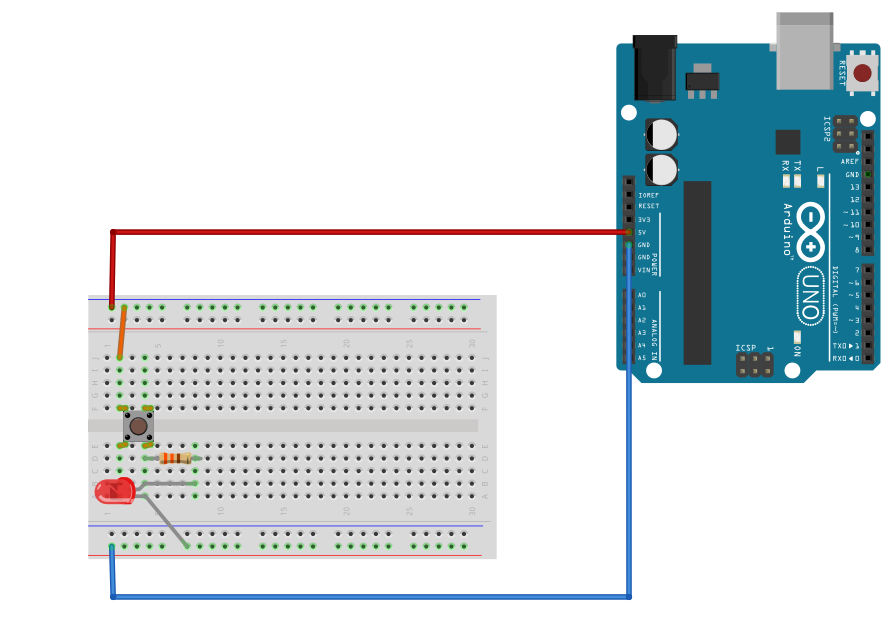
\includegraphics[width=7.0cm]{images/kadai2-1-6_ブレッドボード.png}
\caption{スイッチを用いたLED点灯回路の配線図}
\label{fig:2-1-6bread}
\end{center}
\end{figure}

\begin{figure}[H]
\begin{center}
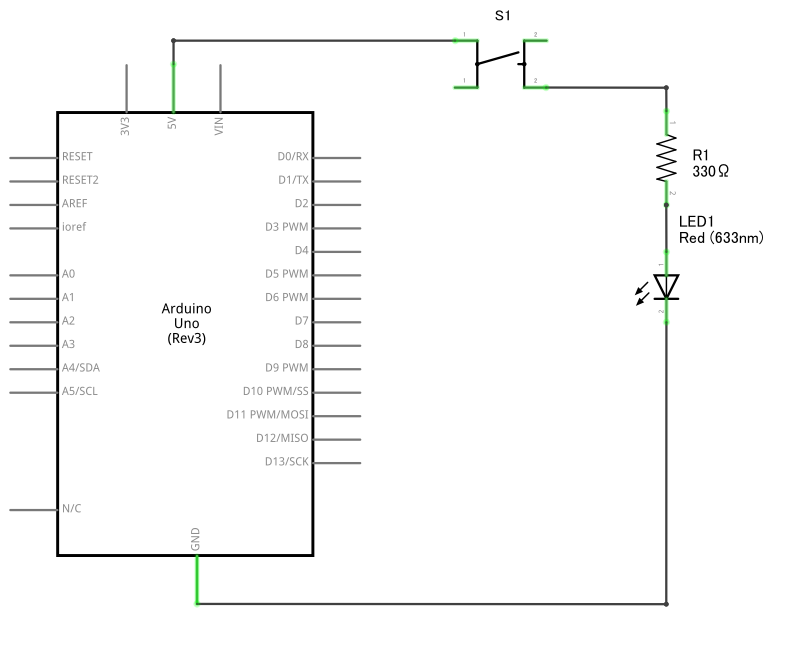
\includegraphics[width=7.0cm]{images/kadai2-1-6_回路図.png}
\caption{スイッチを用いたLED点灯回路の回路図}
\label{fig:2-1-6kairo}
\end{center}
\end{figure}

実験\ref{subsec:switch}で作成したタクトスイッチを2つ用いたLED点灯回路で表\ref{table:and}を満たすもののブレッドボードの配線図を以下図\ref{fig:2-1-7-and-bread}に,回路図を図\ref{fig:2-1-7-and-kairo}にそれぞれ示す.

\begin{figure}[H]
\begin{center}
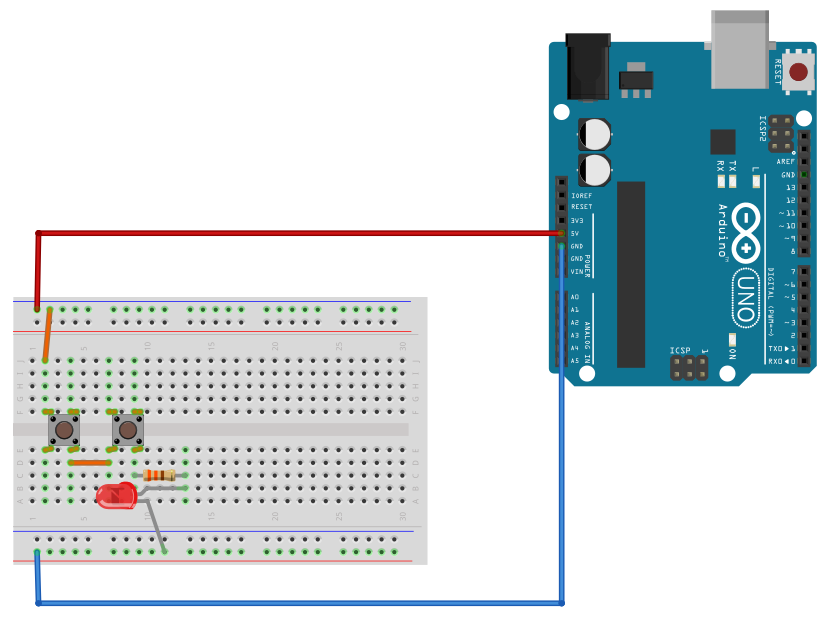
\includegraphics[width=7.0cm]{images/kadai2-1-7-AND_ブレッドボード.png}
\caption{スイッチを2つ用いたLED点灯回路の配線図(条件1)}
\label{fig:2-1-7-and-bread}
\end{center}
\end{figure}

\begin{figure}[H]
\begin{center}
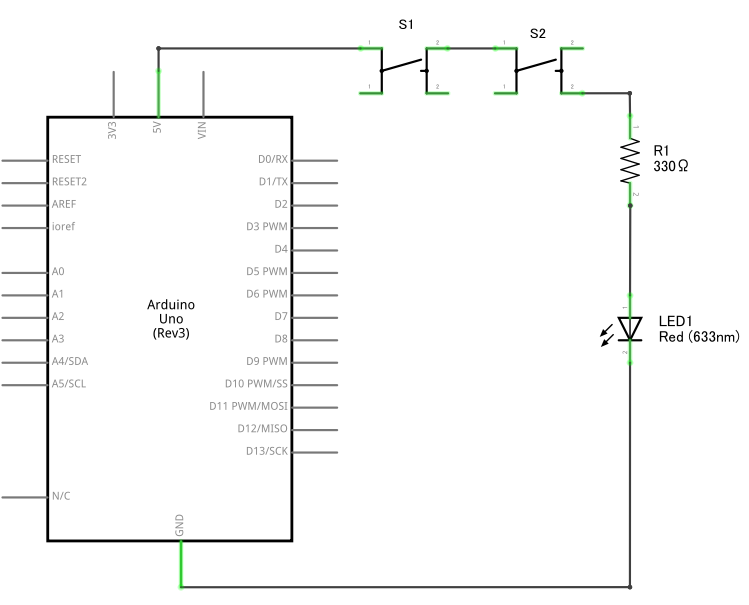
\includegraphics[width=7.0cm]{images/kadai2-1-7-AND_回路図.png}
\caption{スイッチを2つ用いたLED点灯回路の回路図(条件1)}
\label{fig:2-1-7-and-kairo}
\end{center}
\end{figure}

表\ref{table:and}からこの回路の論理構成はAND回路を意味していると考えられる.\\
また,実験\ref{subsec:switch}で作成したタクトスイッチを2つ用いたLED点灯回路で表\ref{table:or}を満たすもののブレッドボードの配線図を以下図\ref{fig:2-1-7-or-bread}に,回路図を図\ref{fig:2-1-7-or-kairo}にそれぞれ示す.

\begin{figure}[H]
\begin{center}
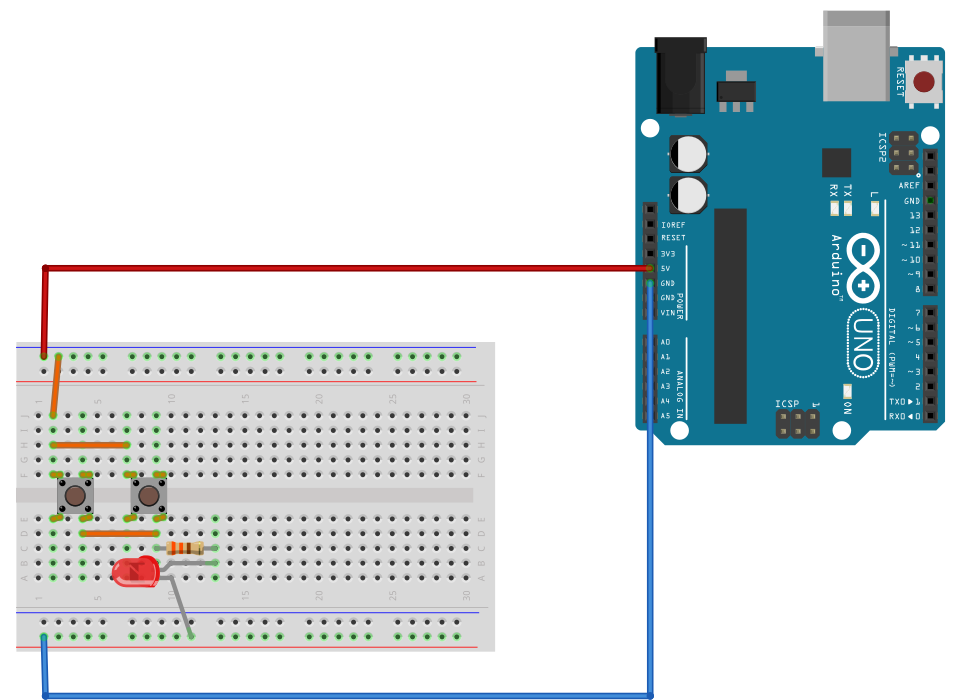
\includegraphics[width=7.0cm]{images/kadai2-1-7-OR_ブレッドボード.png}
\caption{スイッチを2つ用いたLED点灯回路の配線図(条件2)}
\label{fig:2-1-7-or-bread}
\end{center}
\end{figure}

\begin{figure}[H]
\begin{center}
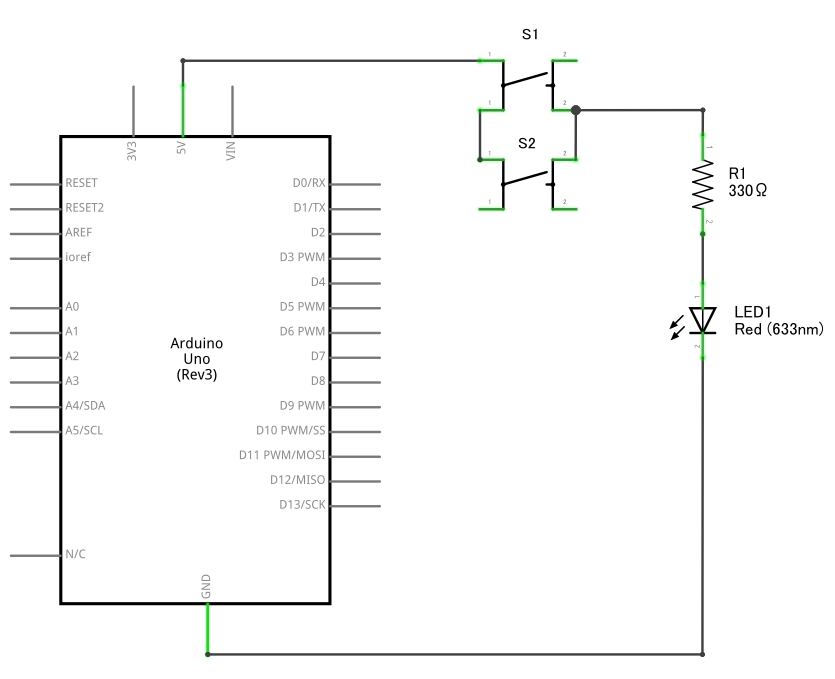
\includegraphics[width=7.0cm]{images/kadai2-1-7-OR_回路図.png}
\caption{スイッチを2つ用いたLED点灯回路の回路図(条件2)}
\label{fig:2-1-7-or-kairo}
\end{center}
\end{figure}

表\ref{table:or}からこの回路の論理構成はOR回路を意味していると考えられる.
\subsection{[発展課題2.1.1]合成抵抗}
実験\ref{subsec:hatten1}で作成した合成抵抗の回路図を以下図\ref{fig:gouseihatten}に示す.
ここで,合成抵抗の計算には式\ref{eq:gouseihatten}を用いた.

\begin{eqnarray}
R&=&R_1+\frac{R_2R_3}{R_2+R_3} \nonumber \\
R&=&330+\frac{1000\times510}{1000+510}=667.7...
\label{eq:gouseihatten}
\end{eqnarray}

\begin{figure}[H]
\begin{center}
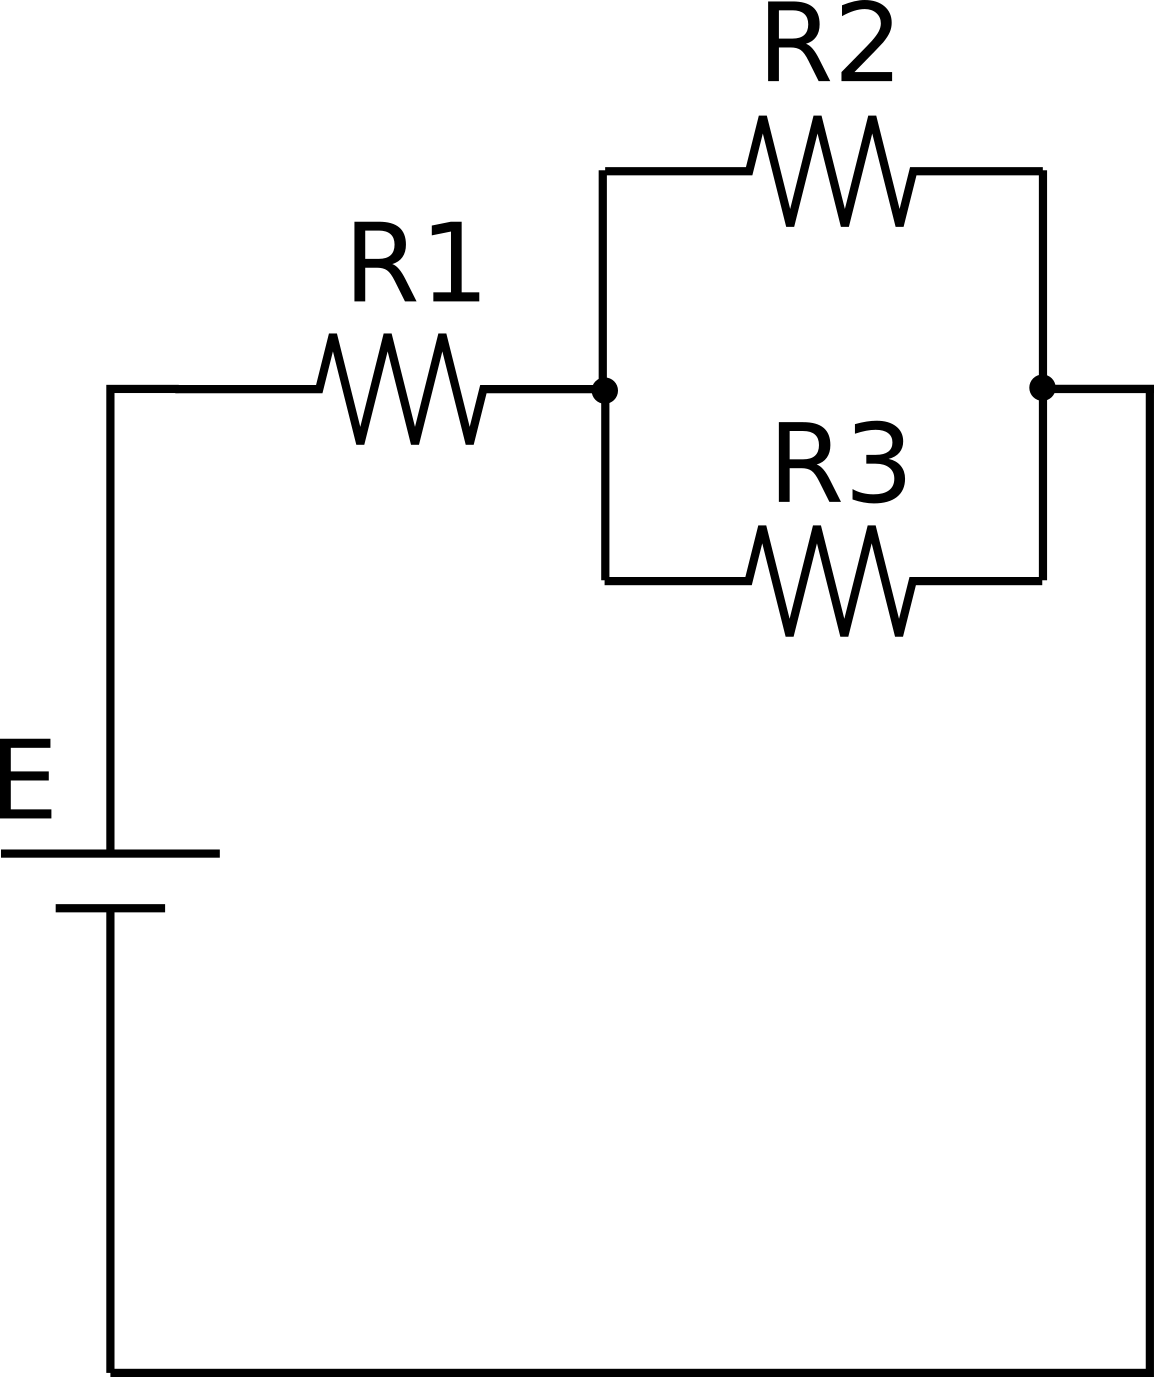
\includegraphics[scale=0.4]{images/合成抵抗.png}
\caption{合成抵抗の回路図}
\label{fig:gouseihatten}
\end{center}
\end{figure}

また,実験\ref{subsec:hatten1}で作成した合成抵抗を用いたLED点灯回路のブレッドボードの配線図を以下図\ref{fig:hatten2-1-1-bread}に,回路図を図\ref{fig:hatten2-1-1-kairo}にそれぞれ示す.

\begin{figure}[H]
\begin{center}
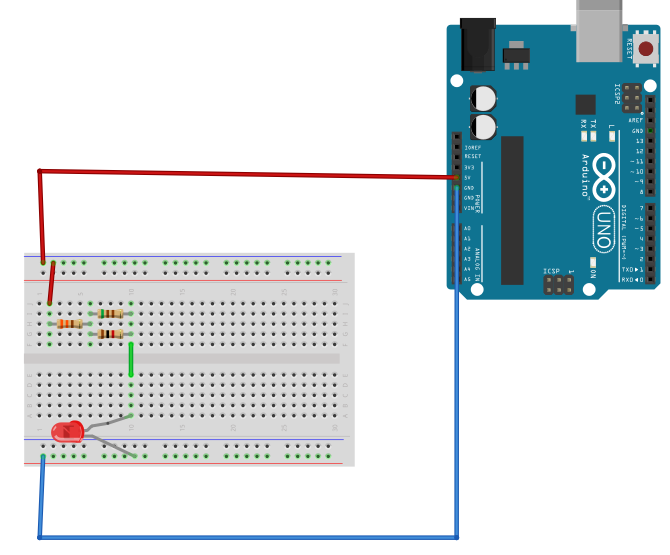
\includegraphics[width=7.0cm]{images/hatten2-1-1_ブレッドボード.png}
\caption{合成抵抗を用いたLED点灯回路の配線図}
\label{fig:hatten2-1-1-bread}
\end{center}
\end{figure}

\begin{figure}[H]
\begin{center}
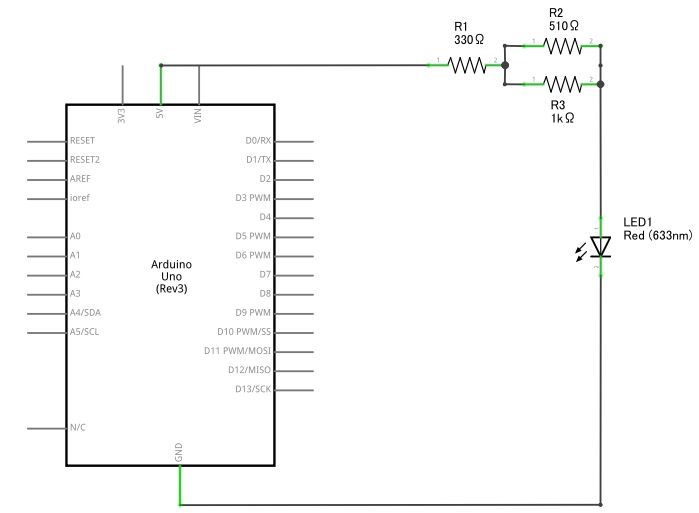
\includegraphics[width=7.0cm]{images/hatten2-1-1_回路図.png}
\caption{合成抵抗を用いたLED点灯回路の回路図}
\label{fig:hatten2-1-1-kairo}
\end{center}
\end{figure}

\subsection{[発展課題2.1.2]RGBフルカラーLEDの点灯}
実験\ref{subsec:hatten2}で作成したRGBフルカラーLEDの発光色を以下表\ref{table:rgbled}に示す.ブレッドボードの配線図を以下図\ref{fig:hatten2-1-2-bread}に,回路図を\ref{fig:hatten2-1-2-kairo}に示す.

\begin{table}[H]
\centering
\caption{RGBLEDの発光色}
\label{table:rgbled}
\begin{center}
\begin{tabular}{c|c|c|c}
\hline \hline
SW1 & SW2 & SW3&LEDの発光色\\ \hline
ON&ON&ON&白\\
ON&ON&OFF&マゼンタ\\
ON&OFF&ON&イエロー\\
ON&OFF&OFF&赤\\
OFF&ON&ON&シアン\\
OFF&ON&OFF&青\\
OFF&OFF&ON&緑\\
OFF&OFF&OFF&点灯なし\\ \hline
\end{tabular}
\end{center}
\end{table}

\begin{figure}[H]
\begin{center}
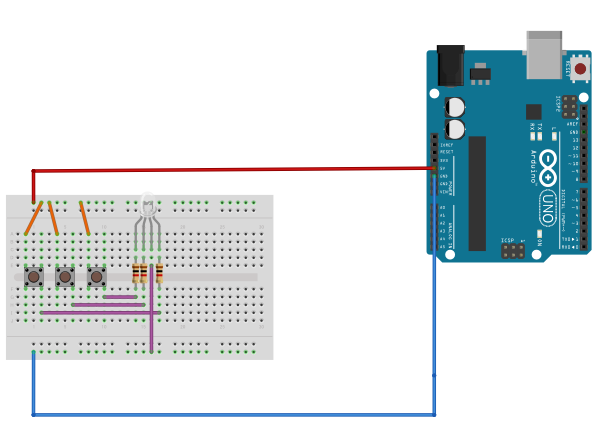
\includegraphics[width=7.0cm]{images/hatten2-1-2_ブレッドボード.png}
\caption{RGBフルカラーLEDの発光回路の配線図}
\label{fig:hatten2-1-2-bread}
\end{center}
\end{figure}

\begin{figure}[H]
\begin{center}
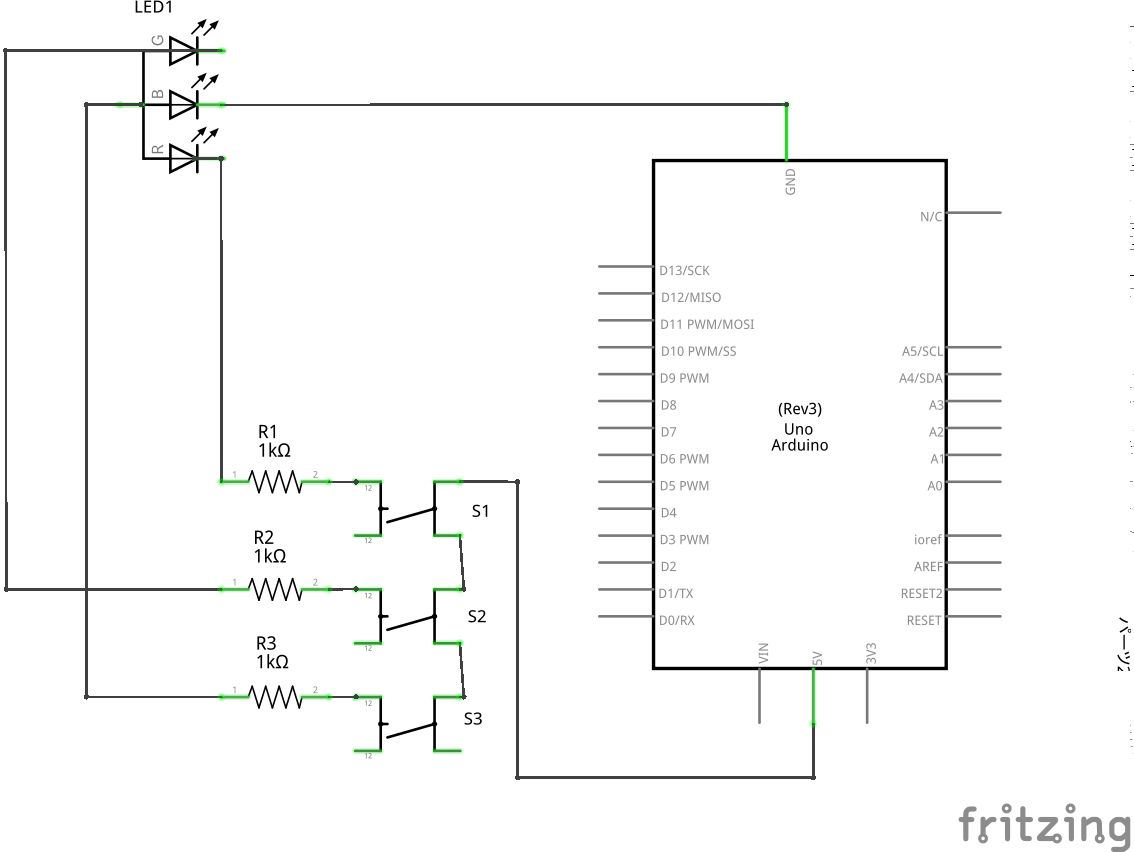
\includegraphics[width=7.0cm]{images/hatten2-1-2_回路図.png}
\caption{RGBフルカラーLEDの発光回路の回路図}
\label{fig:hatten2-1-2-kairo}
\end{center}
\end{figure}

発光色が変化したのはそれぞれ赤緑青の3色から何種類かの色が混ざったためだと考えられる.例えば赤と青のLEDがONの時はそれが混ざりマゼンタとなる.
\section{回路実装の報告}
ブレッドボード上で回路を実装することは高専時代に何度もしたことがあったので特に問題なく実験を進めることができた.ただ,LEDのアノードカソードの区別はリード線の長さでしか判断したことがなかったので他の判断方法を知れてよかった.

\end{document}